\documentclass[12pt]{article}
  \usepackage[francais]{babel}
  \AddThinSpaceBeforeFootnotes % à insérer si on utilise \usepackage[french]{babel}
  \FrenchFootnotes % à insérer si on utilise \usepackage[french]{babel}
  \usepackage[T1]{fontenc}
  \usepackage[utf8]{inputenc}
  \usepackage{graphicx}
  \usepackage[left=2.5cm,right=2.5cm,top=2.5cm,bottom=2.5cm]{geometry}
  \usepackage{array}
  \usepackage{booktabs}
  \usepackage[squaren,Gray]{SIunits}  % Unité ex: $\unit{5 \cdot 10^{-6}}{\meter}$
  \usepackage{colortbl}               % Pour les couleur des cellules (tableau)
  \usepackage{amsmath}				  % Pour les formules mathématiques
  \usepackage{upgreek}                % Pour les lettres greque
  %\usepackage{fullpage}	          % plus petites marges
  \usepackage{verbatim}				  % Pour de long commentaires
  \usepackage[lofdepth,lotdepth]{subfig}       % Faire des sous-figures
  \usepackage{url}
  \usepackage{colortbl}               % pour les couleur des cellules (tableau)
  \usepackage{indentfirst}
  \usepackage{multirow}
  \usepackage{xfrac}
  \usepackage{wrapfig}
  \usepackage{enumitem}               % Liste personnalisée
  \frenchbsetup{StandardLists=true}   % Empêche conflits entre enumitem et babel
  \usepackage{placeins}   % place une barrière pour que l'image/table soit derrière \FloatBarrier
  \usepackage{lastpage} 
  \usepackage{titling}
  \usepackage{lmodern}
  \usepackage{booktabs}
  \usepackage{etoolbox}
  \usepackage[most]{tcolorbox}
  
  
  %Change la taille de police
  \newcommand\ChangeRT[1]{\noalign{\hrule height #1}}
  
\graphicspath{{images/}}

  
  %Création  d'une nouvelle commande pour faire référence à une Figure
  %Exemple : \appelFigure{schema} donne : Figure 1 (en italique)
  \newcommand{\appelFigure}[1]{
    \textit{Figure \ref{#1}}
  }
      
  %%Création commande pour insérer image avec nom de figure directement
  %\newcommand{nomDeTaCommande}[nombreArguments]{CodeLaTeX}
  %\insertImage[position]{image_path}{scale}{Titre_figure}{label}
  \newcommand{\insertImage}[5][center]{
      \begin{#1}
      \includegraphics[scale=#3]{#2}
      \captionof{figure}{#4} 
      \label{#5}
      \end{#1}
  }

  % Affichage des frames pour commande cisco
  \newtcblisting{cisco}[1][]{size=fbox, listing only, listing options={style=tcblatex,basicstyle=\ttfamily\scriptsize,tabsize=2,language=sh},title=#1}

  %En-tête et pied de page personalisé
  \usepackage{fancyhdr}
  \pagestyle{fancy}
  \fancyhf{}
  \setlength\parindent{0pt} %Supprime les alinéa
  \setlength{\parskip}{8pt} %Augmente l'espace entre paragraphe
  %Bottom numbering page
  \renewcommand{\headrulewidth}{1pt}
  \fancyhead[L]{
\includegraphics[scale=.2]{heia-fr-logo.png}}
  \fancyhead[R]{\theauthor}
  
  \renewcommand{\footrulewidth}{1pt}
  \fancyfoot[R]{\textbf{Page \thepage\ sur \pageref{LastPage}}} 
%  \fancyfoot[L]{\leftmark}

  \setlength\parindent{0pt} %Supprime les alinéa
  \setlength{\parskip}{8pt} %Augmente l'espace entre paragraphe


\title{Système Embarqués II, Journal, TP.04:\\ Mise en oeuvre d'un timer hardware en C}
\author{\textsl{Marc} \textsc{Roten} \\ \textsl{Sven} \textsc{Rouvinez}}
\date{}

\begin{document}
    \begin{titlepage}
        \begin{center}
            
\includegraphics[scale=.3]{heia-fr-logo.png}\\[1.3cm]
            
            \rule{\linewidth}{0.3mm} \\[0.3cm]
            {\huge \bfseries Système embarqués \\[0.5cm]} 
           % {\Large Effet photoélectrique}\\[0.2cm]
            \rule{\linewidth}{0.3mm} \\[0.8cm]
            \noindent
            \begin{minipage}[t]{0.4\textwidth}
                \begin{flushleft} \large
                    \emph{Auteurs :}\\
                    \theauthor
                \end{flushleft}
            \end{minipage}
            \begin{minipage}[t]{0.4\textwidth} 
                \begin{flushright} \large
                    \emph{Professeur:}\\
                    \textsl{Daniel} \textsc{Gachet}\\ 
                \end{flushright} 
                \vfill
            \end{minipage}\\[1.3cm]
            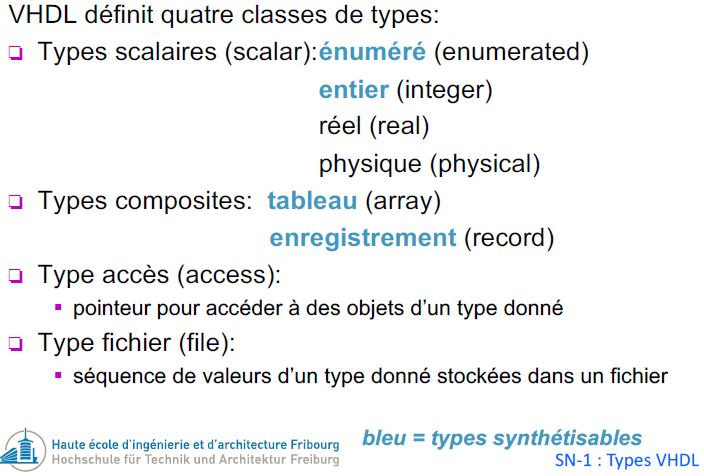
\includegraphics[scale=0.6]{1.JPG}\\[1.5cm]
            \vspace*{1\baselineskip}
            \today \\[0.7cm]
        \end{center}
    \end{titlepage}
    \tableofcontents
    \clearpage
% \insertImage{Img/1.PNG}{echelle pour l'image (source = 1)}{texte dessous l'image}{référence vers l'objet}
\section{Heure de travail}
12 heures

\section{Introduction}
Dans ce travail-ci, nous devrons utiliser un nouveau composant, le DMTIMER, et d'autres composants tels que les boutons et l'écran LED. Le but avec ce DMTIMER est de faire un minijeu dont le but sera de tester nos reflexes. On devra presser le bouton S2, et dès que le signal re relâcher le bouton S2 apparaît, on relâche le dit-bouton et la différence de temps entre les deux sera le temps que l'on affichera sur le LCD.
\section{Synthèse}

\paragraph{Sven}
\begin{itemize}
   \item TODO
\end{itemize}

\paragraph{Marc}
\textbf{\textit{Acquis}}
\begin{itemize}
   \item Découpage et refléxion d'un problème grâce à une machine d'état déterministe (FSM).
   \item Lecture de documentation et compréhension du fonctionnement à partir de cette dite documentation.
   \item Compréhension du fonctionnement de DMTIMER des boutons et du display LCD.
   \item utilisation de la fonction Debug d'Eclipse sur notre BeagleBone.
\end{itemize}
 

\section{Quelle est la signification du qualificatif volatile et quelle est son utilité quand il est associé à un pointeur ?}
Permet d'indiquer au compilateur de ne pas faire d'optimisation \\
L'utilité de lier avec un pointer et de ne pas dépendre de l'exécution du code pour que la valeur change, dans le cas de notre compteur, par exemple, même si le processus travaille sur autre chose, notre timer voa continuer à s'incrémenter
 
\section{Comment sont placés les champs (membres) d’une structure dans la mémoire ?}
De façon continue selon la taille du type choisit

\section{Comment peut-on efficacement définir les registres d’un contrôleur de périphérique situés dans l’espace d’adressage du µP ainsi que leur contenu en C?}
En utilisant des struct
\begin{lstlisting}
    struct timer_reg {
        uint32_t tidr;    //00
        uint32_t res1[3];  //04--0f
        uint32_t tiocp_cfg;  //10
        uint32_t res2[3];   //14--1F
        uint32_t irq_eoi;
        uint32_t irqstatus_raw;
        uint32_t irqstatus;
        uint32_t irqenable_set;
        uint32_t irqenable_clr;
        uint32_t irqwakeen;
        uint32_t tclr;
        uint32_t tcrr;
        uint32_t tldr;
        uint32_t ttgr;
        uint32_t twps;
        uint32_t tmar;
        uint32_t tcar1;
        uint32_t tsicr;
        uint32_t tcar2;
    };      
\end{lstlisting}

\section{Comment peut-on accéder ces registres ?}
En affectant une variable static volatile\\
Exemple: \texttt{volatile struct timer_reg* ctrl = dmtimer[timer];}


\begin{lstlisting}
    static volatile struct timer_reg* dmtimer[] = {
		(volatile struct timer_reg*) 0x48040000,
		(volatile struct timer_reg*) 0x48042000,
		(volatile struct timer_reg*) 0x48044000,
		(volatile struct timer_reg*) 0x48046000,
		(volatile struct timer_reg*) 0x48048000,
		(volatile struct timer_reg*) 0x4804A000 
    };

    uint32_t dmtimer1_get_counter(enum dmtimer_timers timer){
		volatile struct timer_reg* ctrl = dmtimer[timer];
		return ctrl->tcrr;
    }
\end{lstlisting}

\section{Comment générer des nombres aléatoires ?}
Cette fonction permet de générer des nombres aléatoire selon un intervalle donné
\begin{lstlisting}
rand();
uint32_t random_time() {
return random() % ((MAX_VALUE_TIMER + MIN_VALUE_TIMER) + 1)
                  + MAX_VALUE_TIMER;

}
\end{lstlisting}

\section{A la fréquence maximale (24MHz), le compteur du timer ne permet de compter le temps que sur un intervalle de 3 minutes environ. Décrivez l'algorithme à mettre en place si l'on souhaite compter sur plusieurs années avec la même granularité}

\section{Conclusion}

On a pu au travers de ce TP, concevoir les blocs DMTIMER et rajouter les fonctions displayString et displayChar dans notre fichier display.c. Ce TP s'est bien passé et était bien documenté.

\end{document}
